\begin{figure*}[t!]
    \centering
    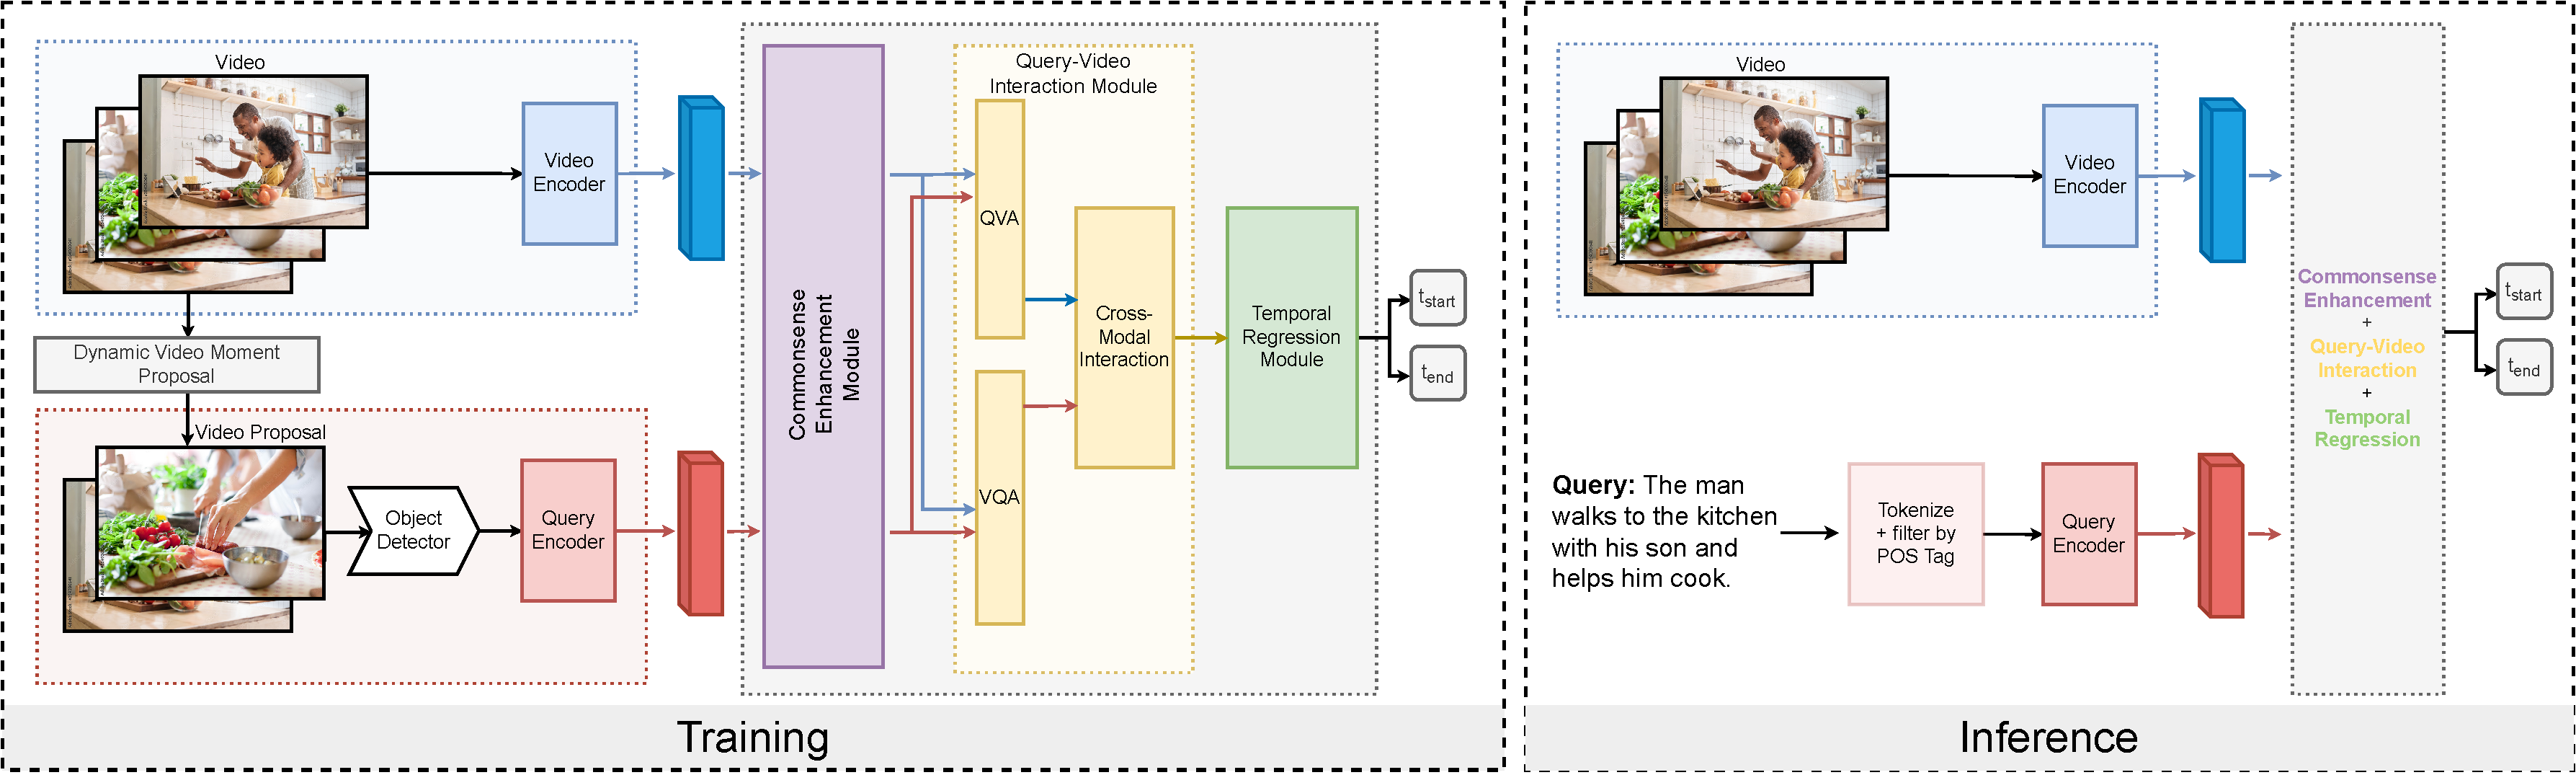
\includegraphics[width=0.95\textwidth]{figures/figure_files/ApproachFull.pdf}
    \caption{\modelname consists of a \textbf{\textcolor{Cerulean}{Video Encoder}} and a \textbf{\textcolor{Red}{Query Encoder}}, the proposed \textbf{\textcolor{RoyalPurple}{Commonsense Enhancement}}, \textbf{\textcolor{Golden}{Cross-modal (video-query) Interaction}}, and a \textbf{\textcolor{ForestGreen}{Temporal Regression}} module. During training, \modelname utilizes a Dynamic Video Moment Proposal module to extract a video moment span \(V_{\text{span}}\) and an off-the-shelf object detector to detect objects (nouns) in \(V_{\text{span}}\). During inference, the given natural language query is converted to a simplified query using a part-of-speech tagger. }
    \label{fig:approach}
\end{figure*}